\subsection{Preliminaries}

Among the three types of attributes that exist in the graph:
\bit
    \item node attributes (e.g., node identity, number of neighbors),
    \item edge attributes (e.g., edge identity, edge weights), and
    \item global attributes (e.g., number of nodes, longest path),
\eit
the objective of the project is to complete recipes and classify cuisine aligns with learning attributes of nodes, especially those of ingredients.
The provided dataset possesses an apparent heterogeneity as visualized in Figure \ref{fig:tripartite}.
In the graph's global scope, ingredient nodes can be considered target nodes, while recipe nodes and cuisine nodes can be considered context nodes.

\begin{figure}[btp!]
    \centering
    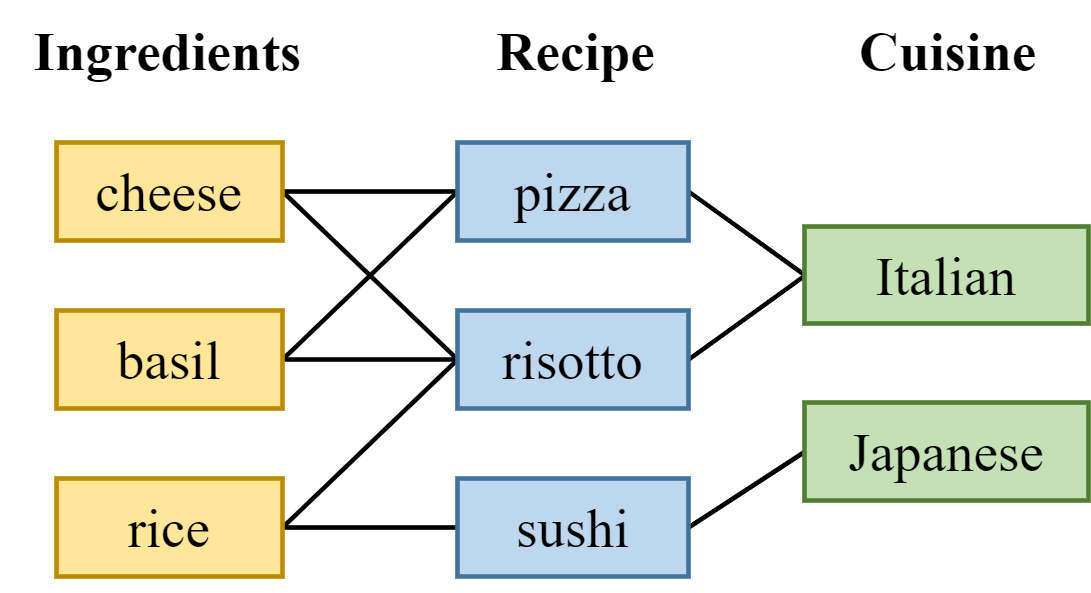
\includegraphics[width=0.6\linewidth]{FIG/tripartite.png}
    \caption{\label{fig:tripartite}Simplified example of constructed graph.}
\end{figure}

\subsection{MultiSAGE}

Our method includes the idea from MultiSage, a graph convolutional network for a recommender system.
The MultiSAGE\cite{10.1145/3394486.3403293} is a GCN engine with contextual information, modeling interactions between target nodes and context nodes in the multipartite network.
The key improvements of MultiSAGE from PinSAGE are \emph{contextual masking} and \emph{contextual attention}.

Contextual masking aggregates the target embeddings $\mathbf{z}_t$ based on context embeddings $\mathbf{z}_c$ as following equation.
\begin{equation}
    \mathbf{z}_{t|c} = \mathbf{z}_t \otimes \mathbf{z}_c
\end{equation}
Since the last embedding layer of $\mathbf{z}_c$ is the ReLU activation function, which sets dimensions with negative values as zeros, the target embeddings' irrelevant dimension is masked out by the corresponding context. This relational operation has intuitive geometrical meanings, and has shown empirical predominancy over popular operations such as summation $\mathbf{z}_t \oplus \mathbf{z}_c$ and dense neural network $\text{RELU}(\mathbf{W}_p(\mathbf{z}_t \otimes \mathbf{z}_c) + \mathbf{b}_p)$.

Contextual attention accounts for the context-wise dynamic impact of neighbor nodes with regard to the ego node. The attention of edge is jointly computed by the ego-context-neighbor relationship as follows.
\begin{equation}
\begin{split}
    & \alpha(v, o, u) = \\
    & \frac{\exp\left(\tau(\mathbf{a}^T[\mathbf{W}_{at}\mathbf{z}_t(v) \odot \mathbf{W}_{ac}\mathbf{z}_c(o) \odot \mathbf{W}_{at}\mathbf{z}_t(u)])\right)}{\sum\limits_{\substack{u' \in \mathcal{N}_v,\\o' \sim (v, u')}}\exp\left(\tau(\mathbf{a}^T[\mathbf{W}_{at}\mathbf{z}_t(v) \odot \mathbf{W}_{ac}\mathbf{z}_c(o') \odot \mathbf{W}_{at}\mathbf{z}_t(u')])\right)}
\end{split}
\end{equation}
Here, $\mathbf{W}_{at}$ and $\mathbf{W}_{ac}$ are the learnable parameters for target embedding and context embedding, respectively. The multi-head attention mechanism is used to aggregate contextualized embedding as follows:
\begin{equation}
    \mathbf{z}_{\mathcal{N}_v}(x) = \sigma \left( \frac{1}{D} \sum_{d=1}^{D} \sum_{u \in \mathcal{N}_v, o \sim (v, u)} \alpha^{(d)}(v, o, u) \mathbf{z}_{t|c}(x, o) \right),
\end{equation}
where $\sigma$ is a sigmoid function.

The training objective is a max-margin ranking described as follows,
\begin{equation}
    \mathcal{J}(v_q, v_p, v_n) = \max\{ 0, \mathbf{h}_{v_q}^T \mathbf{h}_{v_n} - \mathbf{h}_{v_q}^T \mathbf{h}_{v_p} + \delta \},
\end{equation}
where $\delta$ is a margin hyper-parameter. The $v_q, v_p, v_n$ corresponds to the query node, positive node and negative node, respectively, sampled from the training data.

The advances of this project from the original MultiSAGE algorithm are three-fold.
\bit
    \item We empirically demonstrate the claim in \cite{10.1145/3394486.3403293} that MultiSAGE can incorporate multiple context types simultaneously during the training and testing phase.
    \item Furthermore, we extend the \emph{level} of context nodes and show that indirect contexts are also effective for learning target features. For example, as depicted in Figure \ref{fig:tripartite}, we utilize indirect context \textit{cuisine} that are not directly connected to target node \textit{ingredients}.
    \item We extend the architecture to perform collaborative filtering and classification over the learned node embeddings.
\eit

\subsection{Graph construction}

\begin{table}[btp!]
    \centering
    \begin{tabular}{ l r l r }
        \toprule
        \multirow{3}{*}{$|V|$} & \multirow{3}{*}{30281}  & $|V_{I}|$  & 6714   \\
                               &                         & $|V_{R}|$  & 23547  \\
                               &                         & $|V_{C}|$  & 20     \\
        \midrule
        \multirow{2}{*}{$|E|$} & \multirow{2}{*}{277006} & $|E_{IR}|$ & 253459 \\
                               &                         & $|E_{RC}|$ & 23547  \\
        \bottomrule
    \end{tabular}
    \caption{\label{tab:graph_size}Some statistics of graph. $|V|$ and $|E|$ are number of nodes and edges in the graph, respectively. $|V_{I}|, |V_{R}|, |V_{C}|$ are number of nodes with type \textit{ingredient}, \textit{recipe}, \textit{cuisine}, respectively. $|E_{IR}|, |E_{RC}|$ are edges between ingredient and recipe, recipe and cuisine, respectively.}
\end{table}

Alongside the structure of the graph, the method for the generation of initial node features is an interesting topic.
Since the name of every ingredient is given, one might use the NLP-based algorithms to extract feature-based embeddings.
However, because given names are relatively short and the graph consists of a relatively small number of nodes, using identity-based embedding is practical and simplifies the network.

% To discuss:
% \subsection{Recipe completion task}
% \subsection{Cuisine classification task}
